%%&program=xelatex
%&encoding=UTF-8 Unicode
% SVN keywords
% $Author$
% $Date$
% $Revision$
% $URL$
\documentclass[a4paper,12pt]{article}  % Comments after  % are ignored
%\usepackage{hyperref}                 % For creating hyperlinks in cross references
%
\usepackage{ifxetex}% for XELATEX, or PDFlatex
\usepackage{ifplatform} 
%
\ifxetex
	\usepackage{polyglossia} \setmainlanguage{portuges}
	\usepackage{fontspec}
	\ifwindows
		\setmainfont[Ligatures=TeX]{Garamond}
		\setsansfont[Ligatures=TeX]{Gill Sans MT}
		\setmonofont[Scale=0.95]{Courier}
	\fi
	\iflinux
		\setmainfont[Ligatures=TeX]{Linux Libertine O}
		\setsansfont[Ligatures=TeX,Scale=MatchLowercase]{Linux Biolinum}
		\setmonofont[Scale=MatchLowercase]{Courier}
	\fi
	\ifmacosx
	% add settings
	% Use xelatex -no-shell ...
	\fi
	\usepackage{xcolor,graphicx} 
\else
	\usepackage[portuguese]{babel}
	%\usepackage[latin1]{inputenc}
	\usepackage[utf8]{inputenc}
	\usepackage[T1]{fontenc}
	\usepackage{graphics}                 % Packages to allow inclusion of graphics
	\usepackage{color}                    % For creating coloured text and background
\fi

\usepackage{enumitem}
\setlist{nolistsep}

\usepackage{amsmath,amssymb,amsfonts} % Typical maths resource packages
\usepackage[retainorgcmds]{IEEEtrantools}
\usepackage{caption}
\usepackage[bookmarks,colorlinks]{hyperref}

\oddsidemargin 0cm
\evensidemargin 0cm

\pagestyle{myheadings}         % Option to put page headers
                               % Needed \documentclass[a4paper,twoside]{article}
\markboth{{MEFT}}
{{\small\it \protect\input{../../LIFE.txt}}}

\addtolength{\hoffset}{-0.5cm}
\addtolength{\textwidth}{2.5cm}
\addtolength{\topmargin}{-1.5cm}
\addtolength{\textheight}{3cm}

%\textwidth 15.5cm
%\topmargin -1.5cm
\setlength{\parindent}{0pt}
\setlength{\parskip}{1ex  plus  0.5ex  minus  0.2ex}
%\parindent 0.5cm
%\textheight 25cm
%\parskip 1mm


% Math macros
\newcommand{\ud}{\,\mathrm{d}} 
\newcommand{\HRule}{\rule{\linewidth}{0.5mm}}

\author{Prof. Bernardo B. Carvalho} 

%%%%, Bernardo Brotas Carvalho\\bernardo@ipfn.ist.utl.pt} 
\date{ Outubro 2012} 

\begin{document} 

	
\includegraphics[width=0.2\textwidth]{../../logo-ist}%\\[1cm]  %%  Logo_IST_color

	\HRule \\[0.5cm]
	{ \huge \sf  \textsc{Dispersão da Luz por um Prisma}} \\[0.4cm] % \bfseries 
%	{ \huge \sf  \textsc{Construções Geométricas em Lentes Delgadas (aproximação paraxial)} }\\[0.4cm] % \bfseries 
	{ \large \bfseries Indice de refração, poder dispersivo e poder de resolução do vidro pelo método do desvio mínimo}\\
%	{ \large \bfseries Procedimento Experimental}\\
	\HRule \\%[0.5cm]

\section{\sf Objectivo do trabalho}
Com este trabalho pretende-se efetuar um estudo da dispersão da luz através de um prisma de vidro. Através do conceito de ângulo de desvio mínimo, será determinada a variação do índice de refração do prisma com o comprimento de onda. Uma vez conhecido o índice de refração, serão calculadas duas grandezas associadas, o poder dispersivo e o poder de resolução.

\begin{figure}[h!b]  \centering 
	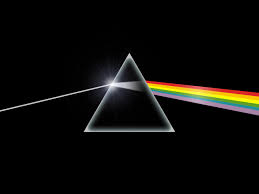
\includegraphics[width=0.55\textwidth]{darkside}
	\caption{A famosa capa do LP ``Dark Side of the Moon" dos Pink Floyd de 1973 ilustra  o fenómeno de dispersão pelo prisma, que foi inicialmente  analisado por Newton.\label{fig:darkside}} 
\end{figure}

\section{\sf Princípio do método}
Um prisma de um meio transparente, homogéneo e isotrópico de índice de refração $n$, quando colocado no percurso de um feixe luminoso incidente produz um desvio angular $\delta$ no feixe emergente que depende do ângulo de incidência, $i_1$. Pode provar-se que a função desvio angular $vs$ comprimento de onda $\lambda$ apresenta um ponto de estacionariedade (i.e., derivada nula) que é um mínimo se $n > 1$.\footnote{Ver Apêndice 2.}
Mostra-se também que, nessa situação, as direções dos dois feixes são igualmente inclinadas em relação às faces do prisma, i.e.  o ângulo de incidência $i_1$ é igual ao ângulo de transmissão emergente $t_2$ (Figura \ref{fig:desvio}). 
Nesse caso, o índice de refração, $n$, pode ser calculado\footnote{Ver também Apêndice 2.} simplesmente através da expressão seguinte: 

\begin{equation}
	\label{eq:desviomim}
	n= \frac{\sin \left( \frac{\alpha+ \delta_{min}}{2} \right) } {\sin \left(  \frac{\alpha}{2} \right)}  
\end{equation}



%\footnote{A figura tem no entanto um problema na refração na segunda face.}

\begin{figure}[htb]  \centering 
	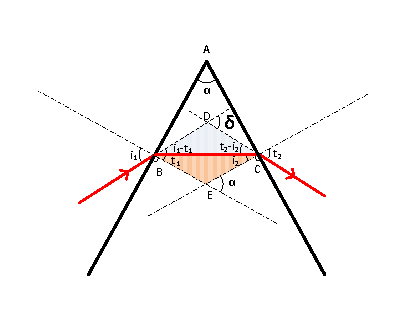
\includegraphics[width=0.6\textwidth]{desvio}
	\caption{Esquema da transmissão do feixe incidente num prisma colocado na plataforma do goniómetro de Babinet. A direção do feixe transmitido desvia-se do ângulo $\delta$ em relação ao feixe incidente. \label{fig:desvio}} 
\end{figure}


em que $\alpha$ e  $\delta_{min}$ são o ângulo do vértice do prisma e o ângulo de desvio mínimo referido, respetivamente. Este desvio mínimo depende do comprimento de onda da radiação incidente, $\lambda$, em virtude de  $n$ depender de $\lambda$. 

\subsection{Poder dispersivo e poder de resolução}
Define-se \emph{poder dispersivo} dum material como a derivada de $n$ em ordem a $\lambda$, e escreve-se  como $\left( \frac{\ud n}{\ud \lambda } \right)$. Como esta função não é constante, deve indicar-se o valor do poder dispersivo relativamente a um determinado valor de comprimento de onda incidente, ou $\left( \frac{\ud n}{\ud \lambda } \right)_{\lambda_i}$ .

O \emph{poder separador} ou \emph{poder de resolução} de um dado instrumento óptico\footnote{\emph{Optical Resolution} em inglês.}, definido como $R_\lambda = \frac{\lambda}{\Delta \lambda} $,  é a capacidade que este possui de permitir que se observem separadamente dois comprimentos de onda muito próximos, afastados de $\Delta \lambda$, na vizinhança de um valor médio $\overline{\lambda}$. Esta grandeza é adimensional e quanto maior for o seu valor, melhor é a resolução do instrumento.

No caso do prisma obtém-se a seguinte expressão para \footnote{Ver derivação no Apêndice 3}.
%, se a fonte é linear e se dispõe paralelamente à aresta do prisma:
 \begin{equation}
	\label{eq:resolu}
	R_\lambda = l\,\left(\frac{\ud n}{\ud \lambda} \right)_\lambda 
\end{equation}

em que $l$ é o \emph{maior percurso} do feixe luminoso no interior do prisma.

Uma \emph{rede de difração}
% (ver apontamentos da Aula Teórica  “Interferência e Difração”)
permite também observar separadamente dois comprimentos de onda muito próximos.
No entanto, para uma rede de difração linear a resolução (além de variar com o comprimento de onda) depende da \emph{ordem de difração}, $m$
 \begin{equation}
	\label{eq:resoludrifa}
	R_{\lambda_{difrac}} = m\,N 
\end{equation}
sendo $N$  o número de linhas da rede \emph{iluminadas} pelo feixe.


\section{\sf A experiência}
\subsection{\sf Equipamento}

\begin{enumerate}
\item Goniómetro de Babinet.
\item Prisma triangular de vidro.
\item Lâmpada espetral de Mercúrio ou Hélio.
\end{enumerate}

No Trabalho anterior colocou-se o prisma na plataforma de modo a poderem observar-se as reflexões nas duas faces polidas (Fig. \ref{fig:angulo}). As direções dos raios refletidos fazem um ângulo $\theta$, que se mediu com o goniómetro e que é o dobro do ângulo principal do prisma $\alpha$.\footnote{Ver Apêndice 1.}  Determinou-se  assim facilmente o ângulo do prisma com uma precisão e exatidão muito melhores do que com um transferidor, por exemplo.

\begin{figure}[tb]  \centering 
	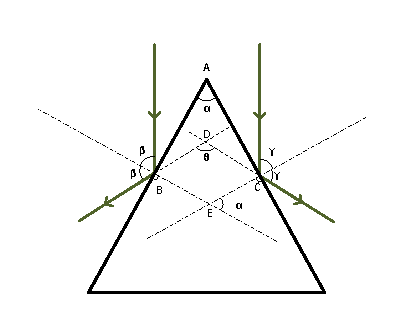
\includegraphics[width=0.6\textwidth]{angulo}
	\caption{Esquema da reflexão do feixe incidente num prisma colocado na plataforma do goniómetro de Babinet. As direções dos dois raios refletidos fazem entre si um ângulo $\theta$ que é o dobro do ângulo $\alpha$ do prisma. \label{fig:angulo}} 
\end{figure}

À partida podia determinar-se  o ângulo $\delta_{min}$ medindo com a objectiva a direção do raio incidente (sem prisma) e a direção do raio emergente que corresponda ao desvio mínimo (Figura \ref{fig:desvio}). No entanto, para compensar as eventuais assimetrias do aparelho devem fazer-se observações para os desvios à esquerda e à direita.
% para os raios que emergem das duas faces que definem o ângulo do prisma. 
Neste cas,o é facil provar que o ângulo formado entre os dois raios emergentes (para a mesma cor) é o dobro do ângulo de desvio, $\delta_{min}$ (não sendo  necessário determinar a direção do raio incidente, $i_1$).
% segundo o ângulo $i_2$ em relação à normal (
% para cada comprimento de onda 


\begin{figure}[tb]  
\centering 
	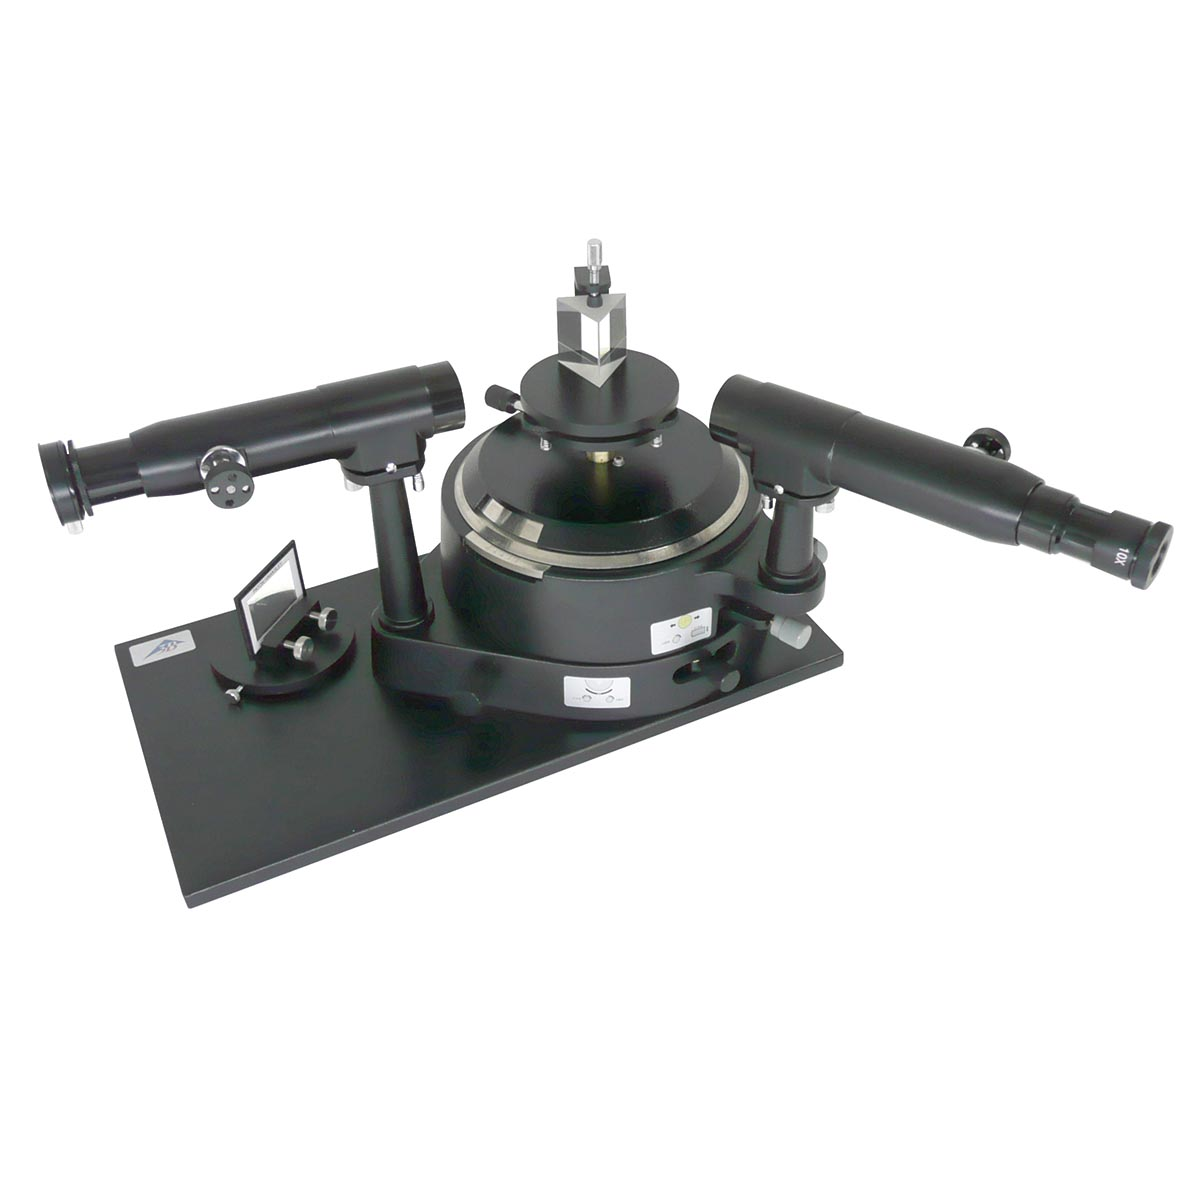
\includegraphics[width=0.55\textwidth]{Espectrometro-Goniometro-S}
	\caption{Fotografia do goniómetro de Babinet utilizado na experiência. \label{fig:spectrometer}} 
\end{figure}


%\begin{figure}[!htb]  
%	\centering 
%	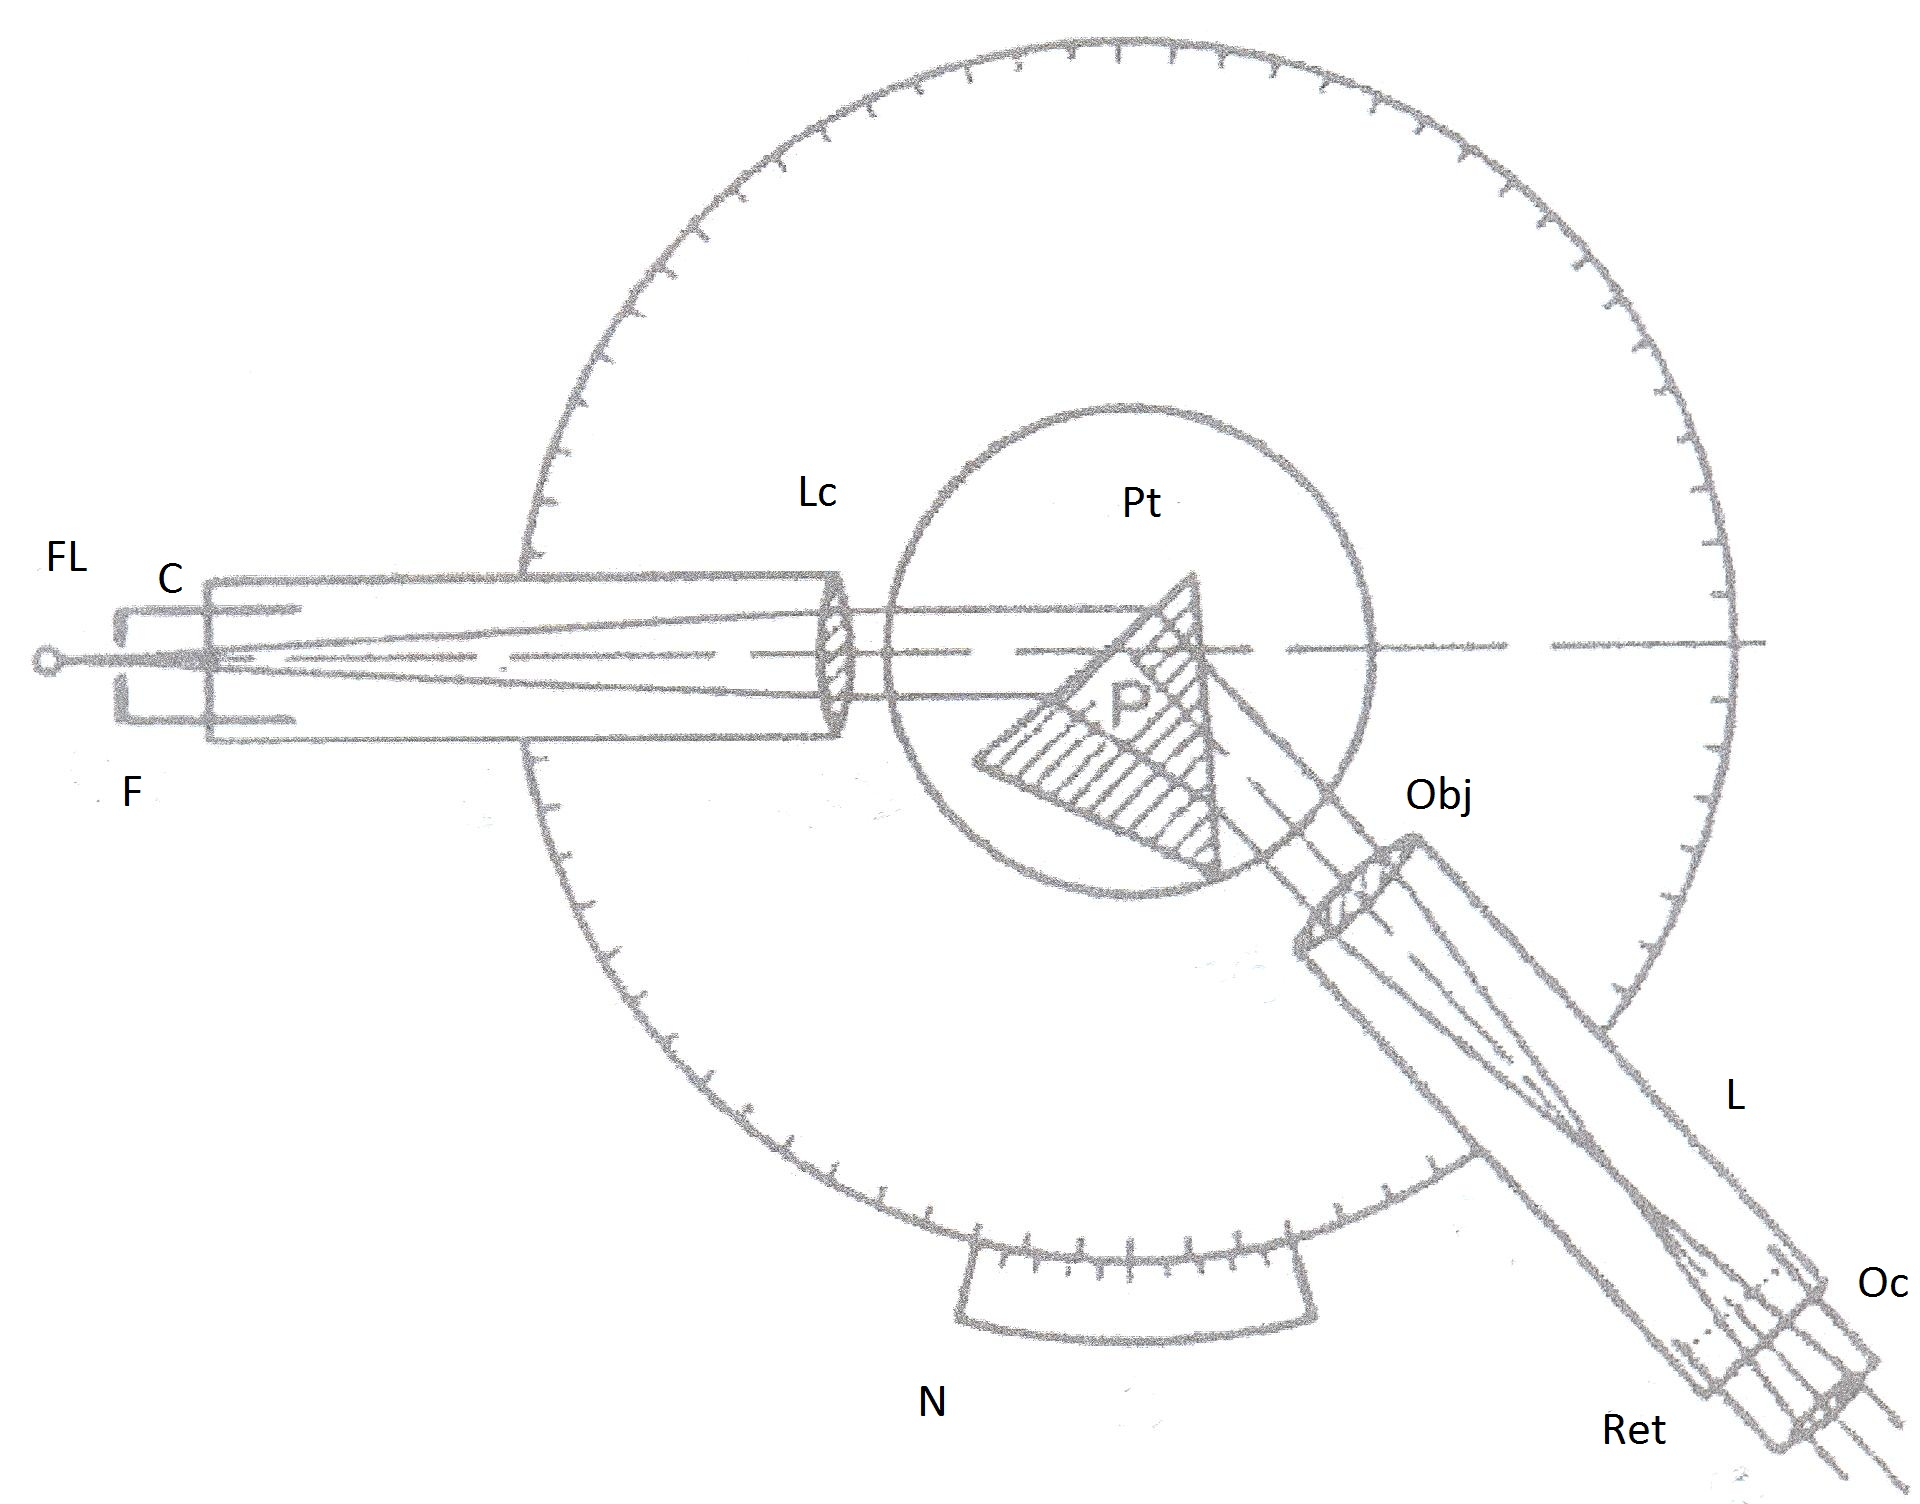
\includegraphics[width=0.55\textwidth]{babinet}
%	\caption{Esquema do Goniómetro de Babinet. Legenda: FL-fonte luminosa, C-colimador, F-fenda, Lc-lente convergente do colimador, Pt-plataforma, %P-Prisma, L-luneta, Obj-objetiva, Oc-ocular, Ret-retículo, N-nónio acoplado à luneta\label{fig:babinet}} 
%\end{figure}


O prisma que se usa é em geral de secção reta triangular (equilátero ou isósceles).
A lâmpada espetral é uma fonte de luz policromática  que contem dois elétrodos situados no interior de um invólucro (vidro em geral) onde existe uma substância “ativa”\footnote{Que dá o nome à lâmpada, e.g. Mercúrio, Hélio, Néon, etc.} em muito pequena quantidade, numa atmosfera rarefeita. A alimentação, em geral é de alta tensão, produz entre os elétrodos uma descarga que vaporiza, excita e ioniza a substância ativa. As diferentes excitações permitem transições radiativas que dão origem à emissão de um feixe constituido por diferentes comprimentos de onda bem definidos e que se encontram muito bem identificados na literatura.\footnote{Pode consultar a extensa base de dados online em  \href{http://physics.nist.gov/asd}{NIST Atomic Spectra Database}.} 

Todas as lâmpadas espetrais emitem no ultravioleta que é nocivo para a pele e e para os olhos dos observadores, mas o vidro no interior do qual se dá a descarga absorve a maior parte destas radiações perigosas. Para ainda reduzir os riscos, a lâmpada tem um invólucro, em geral metálico, apenas com uma abertura para permitir iluminar uma fenda estreita e regulável junto à luneta do goniómetro, que produz uma linha vertical na imagem.  A aresta do triângulo definido pelas superfícies planas onde se produz a reflexão e/ou transmissão deve ficar paralela a esta fenda.

% ~
% \newpage
% \subsection{\sf Questões a responder ANTES da sessão de Laboratório:}
% \begin{enumerate}
% \item Descreva quais os objectivos do Trabalho que irá realizar na sessão de Laboratório. Indique as expressões que irá utilizar para obter as grandezas experimentais, bem como as expressões para calcular as incertezas. Inclua esta parte também no Relatório Impresso. Este irá constituir o ÚNICO meio de consulta na Prova Individual.
% \item Obtenha uma imagem típica da dispersão da Luz Branca num prisma triangular. A partir dessa figura pode concluir que índice de refração, $n(\lambda)$, é uma função crescente ou decrescente?
% \item Nessa figura de dispersão como pode identificar qual é a côr que está na posição de \emph{desvio mínimo}?
% \item Se na montagem de laboratório substituir a lâmpada de descarga pela luz Solar que imagem observaria na luneta do goniómetro?.
% \item O espectro de emissão do Hidrogéneo, na série de Balmer (transição eletrónica de nível $3 \to 2$) tem duas riscas no c.d.o. vermelho, respetivamente a $\lambda = 656.272\, nm$ e $\lambda = 656.2852\,nm$.
% Qual a Resolução mínima de um Instrumento (Espectrómetro) capaz de distinguir estas duas linhas?. Supondo que tem um prisma com aresta de $10\,cm$, calcule o
% o valor absoluto mínimo para $\left(\frac{\ud n}{\ud \lambda} \right)$?
% \end{enumerate}


\section{\sf Protocolo Experimental}

\begin{enumerate}
\item Ligue  a  lâmpada  espetral  e  espere  10  a  15  minutos    até  que  se  estabeleça  o 
equilíbrio térmico no seu interior. 
\item Enquanto espera comece por regular a ótica  do goniómetro tal como descrito no Guia do Trabalho anterior.
\item Verifique o nivelamento horizontal do goniómetro e da plataforma onde vai colocar o prisma com a ajuda de um nível de bolha. 
\item Utilize o valor do ângulo $\alpha$ entre as faces polidas do prisma obtido no trabalho anterior.
\item  Observe agora  a  transmissão  das várias cores  através  do  prisma  com  o  feixe  incidente  numa  das  faces, na posição da Figura \ref{fig:desvio}.  Se o instrumento estiver bem focado deve  observar   uma  série  de 
imagens coloridas da mesma fenda isoladas (riscas), uma por cada comprimento de onda $\lambda$.
\item Escolha duas dessas cores bem afastadas. Rodando o prisma obtenha um conjunto de valores que permita fazer um gráfico dos ângulos de desvio, $\delta(i_1)$, 
em função do ângulo de incidência, $i_1$ e um ajuste polinomial (Nesta fase não precisa de utilizar o nónio da escala de minutos). Pelo gráfico verifique que existe de facto um mínimo no ângulo de desvio,  $ \delta(i_{min})$, mas  que este e o ângulo $i_{min}$ são  diferentes para cada cor.

\item  Em seguida, para medir o desvio mínimo,  \emph{para cada risca}, tem primeiro de colocar o prisma na posição apropriada. Deve portanto olhar pela objectiva e, fixando a risca,  rodar o prisma até observar que o desvio é mínimo.
%Pode finalmente medir os ângulos de desvio, $\delta_{min(esq, dir)}(\lambda)$.
% agora com o nónio e o auxílio  do  parafuso  micrométrico  associado  à  plataforma.  
De seguida,  com  o  parafuso micrométrico associado à luneta, centrar  a imagem  da fenda no retículo e meça o  ângulo  $\delta_{min(esq)}(\lambda)$. Comece por usar todas as cores quando o prisma desvia para o lado esquerdo (cada elemento do grupo deve efectuar as suas medidas). 
\item Repita o ponto anterior, mas para o prisma a desviar o feixe para o lado direito. Calcule os desvio mínimos:
$$\delta_{min}(\lambda) = \frac{|\delta_{esq} -  \delta_{dir}|}{2}$$ 
\item Com os desvio mínimos, e identificando  nas tabelas os valores  dos  comprimentos  de onda das riscas visíveis, calcule o
índice de refração a partir da Eq.~\ref{eq:desviomim} e represente  graficamente a função $n(\lambda)$. Ajuste uma curva polinomial aos pontos obtidos. Através da  estimativa da derivada desta função, calcule o poder dispersivo do vidro para o comprimento de onda médio das 
duas riscas amarelas do sódio ($\overline{\lambda}_{amarel}\approx 589\,nm$). 
\item Faça uma estimativa da maior distância percorrida pelo feixe luminoso no prisma,$l$, (que é aproximadamente o comprimento da aresta) e calcule 
  o  Poder  de  Resolução  do  prisma  para  o comprimento de onda $\overline{\lambda}_{amarel}$ referido  no  ponto  anterior. 
%Compare este valor com o que obteria se usasse o mesmo feixe com uma rede de difração 
%de 600 linhas por milímetro. 
\item Substitua no centro da plataforma do goniómetro o prisma por uma rede de difração de 
600 linhas por milímetro. Compare a separação angular, $\Delta \delta_{rede}$, das duas riscas mais próximas 
observadas  com  a  rede  com  a  que  obteve,  para  as  mesmas  riscas,  usando  o  prisma. 
Comente, utilizando a expressão (\ref{eq:resoludrifa}). 

\end{enumerate}

%\newpage
\section*{\sf Apêndices}
\subsection*{\sf A1. Ângulo do Prisma}

Vamos demonstrar que o ângulo $\theta$ entre as direções dos dois feixes reflectidos é o dobro do ângulo do vértice do prisma $\alpha$. Considere-se a incidência nas condições da Figura \ref{fig:angulo}.
A figura plana quadrangular $ABEC$ tem dois ângulos retos: $ABE$ e $ECA$. Assim o ângulo $CAB$, $\alpha$, é suplementar do ângulo $BEC$, e portanto o ângulo externo em $E$ (assinalado na figura) tem o mesmo valor do ângulo do prisma.
Na figura plana quadrangular DBEC está definido um ângulo $\theta$ que é o ângulo formado pelas direções dos raios refletidos na face $AB$ e $AC$. 
Entre este ângulo e os ângulos de incidência $\beta$ e $\gamma$ existe a relação 

 \begin{equation}
	\label{eq:soma}
	2\, \beta  + 2 \, \gamma + \theta = 2 \, \pi
\end{equation}

e entre os ângulos de $DBEC$ 
 \begin{equation}
	\label{eq:soma2}
	\beta  +  \gamma + \theta  + \pi - \alpha= 2 \, \pi
\end{equation}

O sistema destas duas equações permite obter 
 \begin{equation}
	\label{eq:alpha}
	\alpha=  \theta /2 
\end{equation}

\subsection*{\sf A2. Desvio mínimo}
Iremos demonstrar que (i) o feixe para o qual o desvio é mínimo atravessa o prisma simetricamente (isto é, paralelamente à sua base) e (ii) essa configuração corresponde de facto a um mínimo do desvio.

Supondo um prisma que tem um índice de refração $n$ em relação ao meio em que está imerso, na configuração da Figura \ref{fig:desvio}, os feixes que são transmitidos através do mesmo sofrem um desvio $\delta(\lambda)$. Os ângulos  $\alpha$ e de desvio $\delta $  são exteriores respetivamente aos triângulos $BCD$ (em $D$) e $BEC$ (em $E$), e portanto temos


\begin{IEEEeqnarray}{rCl}
\delta &  =  &  (i_1 - t_1) +  (t_2 - i_2) \\
\alpha &  =  &  t_1  + i_2 \label{eq:soma3}
\end{IEEEeqnarray}

o que permite obter a seguinte relação fundamental
 \begin{equation}
	\label{eq:delta}
	\delta   =    i_1  +  t_2  - \alpha 
\end{equation}

Por outro lado, estes ângulos satisfazem a lei de Snell-Descartes da refração (para o feixe de entrada e para o de saída)

 \begin{equation}
	\label{eq:snell}
	n = \frac{\sin i_1}{\sin t_1}  =  \frac{\sin t_2}{\sin i_2}  
\end{equation}

No caso geral o ângulo $\delta$ depende do ângulo de incidência $i_1$ e pode provar-se que a função envolvida tem uma estacionariedade. Para encontrar o \emph{desvio mínimo} $\delta_{min}$, comecemos então por calcular  a derivada de $\delta$ em relação ao ângulo de incidência $i_1$ (expressão \ref{eq:delta}).

 \begin{equation}
	\label{eq:deriv}
	\frac{\ud \delta}{\ud i_1}   =  1 + 	\frac{\ud t_2}{\ud i_1} 
\end{equation}

Obtendo $\sin i_1$ e $\sin t_2$ da relação (\ref{eq:snell}) e calculando também as suas derivadas em ordem a $i_1$ obtemos as duas igualdades
\begin{IEEEeqnarray}{rCl}
\cos i_1 &  =  & n \,\cos t_1 \cdot  \frac{\ud t_1}{\ud i_1} 	\label{eq:deriv2} \\
\cos t_2  \cdot   \frac{\ud t_2}{\ud i_1}  &  =  & n \, \cos i_2  \cdot  \frac{\ud i_2}{\ud i_1} 	\label{eq:deriv3}
\end{IEEEeqnarray}

Atendendo à relação (\ref{eq:soma3}) temos também para a sua derivada
 \begin{equation}
	\label{eq:deriv4}
	\frac{\ud t_1}{\ud i_1}  = - \frac{\ud i_2}{\ud i_1} 
\end{equation}

e combinando (\ref{eq:deriv2}), (\ref{eq:deriv3}) e (\ref{eq:deriv4}) obtém-se
 \begin{equation}
	\label{eq:deriv5}
	\frac{\ud t_2}{\ud i_1}  = - \frac{\cos i_2\,\cos i_1}{\cos t_2\,\cos t_1} 
\end{equation}

e a relação (\ref{eq:deriv}) vem

\begin{equation}
	\label{eq:deriv6}
	\frac{\ud \delta}{\ud i_1}   = 1-  \frac{\cos i_2\,\cos i_1}{\cos t_2\,\cos t_1} 
\end{equation}

Esta função admite um zero para a seguinte condição:
\begin{equation}
	\label{eq:deriv_0}
	{\cos i_2\,\cos i_1}={\cos t_2\,\cos t_1} 
\end{equation}

Atendendo a (\ref{eq:snell}) e à relação entre coseno e seno obtém-se (após alguns cálculos, aqui abreviados)
\begin{equation}
	\label{eq:deriv_1}
	\sin^2 t_1 \cdot  (1 - n^2)  = \sin^2 i_2 \cdot  (1 - n^2)
\end{equation}

que para os ângulos considerados ($\le  \pi/2)$ e para $n\ne 1$ implica que no ponto de estacionariedade de $\delta$ se verificam as seguintes condições de simetria:
\begin{IEEEeqnarray}{rCl}
i_1  &  =  & t_2 = i\\
t_1  &  =  & i_2 = t
\end{IEEEeqnarray}


Ou seja: o ângulo de incidência $i_1$ é igual ao ângulo de saída do prisma $t_2$, e os ângulos de refracção interna $t_1$ e $i_2$ são iguais. Isto implica que o feixe se propaga paralelamente à base do prisma. Obtém-se assim a seguinte expressão para o ângulo de desvio mínimo
\begin{equation}
	\label{eq:deltvmin}
	\delta_{min} = 2\,i- 2\,t = 2\,i - \alpha
\end{equation}

o que permite calcular $t$ a partir do ângulo do prisma ($t = \alpha / 2$) e $i$ a partir do ângulo de desvio mínimo e do ângulo do prisma ($i = (\alpha + \delta_{min} ) / 2$) e consequentemente obter a relação (\ref{eq:desviomim}) para o cálculo do índice de refração:
\begin{equation}
	\sin i = n\sin t \rightarrow n=\frac{\sin(\frac{\alpha + \delta_{min}}{2} )}{\sin(\alpha / 2)}
\end{equation}

Vamos agora provar que este ponto de estacionariedade é efectivamente um mínimo. Para isso, é necessário calcular  $\frac{\ud^2 \delta}{\ud i^2} =0 $ e verificar que é uma quantidade positiva para os valores que anulam a primeira derivada. Aplicando derivada em ordem a $i_1$ à expressão (\ref{eq:deriv6}) obtém-se

\begin{equation}
	\label{eq:d2eriv}
	\frac{\ud^2 \delta}{\ud i_1^2}   =   	\frac{\ud }{\ud i_1} \left(-  \frac{\cos i_2\,\cos i_1}{\cos t_2\,\cos t_1} \right)
\end{equation}

em que todos os argumentos das funções coseno dependem de $i_1$.
Obtém-se quatro parcelas, que são: 

\begin{IEEEeqnarray}{rCl}
 \frac{\cos i_1}{\cos t_2\,\cos t_1} \frac{\ud }{\ud i_1} \cos i_2 &  =  & 
 \frac{\cos i_1}{\cos t_2\,\cos t_1} (-\sin i_2) \frac{\ud i_2}{\ud i_1} 	\label{eq:d2eriv_a}\\
%
 \frac{\cos i_2}{\cos t_2\,\cos t_1} \frac{\ud }{\ud i_1} \cos i_1 &  =  & 
 \frac{\cos i_2}{\cos t_2\,\cos t_1} (-\sin i_1)  \label{eq:d2eriv_b} \\
 \frac{\cos i_2\,\cos i_1}{\cos t_1}  \frac{\ud }{\ud i_1} (\cos t_2)^{-1} &  =  & 
  \frac{\cos i_2\,\cos i_1}{\cos t_1} \sin t_2 (\cos t_2)^{-2} \frac{\ud t_2}{\ud i_1}\label{eq:d2eriv_c}\\
  \frac{\cos i_2\,\cos i_1}{\cos t_2}  \frac{\ud }{\ud i_1} (\cos t_1)^{-1}  &  =  & 
  \frac{\cos i_2\,\cos i_1}{\cos t_2} \sin t_1 (\cos t_1)^{-2} \frac{\ud t_1}{\ud i_1} \label{eq:d2eriv_d}
\end{IEEEeqnarray}

Atendendo a (\ref{eq:deriv2}) e (\ref{eq:deriv4}) substituidos em (\ref{eq:d2eriv_a}) e em (\ref{eq:d2eriv_c}) e a (\ref{eq:deriv5}) substituido em (\ref{eq:d2eriv_d}), as quatro parcelas conduzem respetivamente às expressões seguintes que são simplificadas quando se substitui $n$ (\ref{eq:snell}) e se impõem as condições que foram obtidas para o zero de   $\frac{\ud \delta}{\ud i_1} $ 

\begin{IEEEeqnarray}{rCl}
 \frac{\cos i_1}{\cos t_2\,\cos t_1} (-\sin i_2) \frac{\cos i_1}{n\, \cos t_1}  &  =  & 	
    \frac{\sin^2 t}{\cos^2 t}  \frac{\cos i}{\sin i} \\
%
 \cdots &  =  & -\frac{\sin i}{\cos i} \\
 \cdots &  =  & -\frac{\sin i}{\cos i} \\
 \cdots &  =  & 	  \frac{\sin^2 t}{\cos^2 t}  \frac{\cos i}{\sin i} 
\end{IEEEeqnarray}

Assim obtém-se 

\begin{equation}
	\label{eq:d22e}
	\frac{\ud^2 \delta}{\ud i_1^2}   =   -2 \tan^2 t  \, \frac{1}{\tan i} + 2\tan i = 2 \, \tan i 
	\left(1 - \frac{\tan^2 t}{\tan^2 i} \right)
\end{equation}
Esta expressão é positiva para $ \tan^2 t < \tan^2 i $ o que implica $t < i$ ($i, t \le \pi/2$), i.e. para $n > 1$, e é negativa para $n < 1$. No caso do prisma de vidro imerso no ar tem-se $n > 1$ e portanto a expressão (\ref{eq:d22e}) será positiva, o que confirma que a condição de estacionariedade corresponde a um mínimo.

\subsection*{\sf A3. Poder de resolução do prisma}

Vamos determinar uma expressão geral para o poder de resolução de um prisma. A capacidade de observar separadamente dois comprimentos de onda muito próximos está relacionada com a variação do ângulo de desvio $\delta$ com o comprimento de onda $\lambda$, que se designa por \emph{dispersão angular  } 
$\frac{\ud \delta}{\ud \lambda}$ e que depende do coeficiente de dispersão  $\frac{\ud n}{\ud \lambda}$ na forma  

\begin{equation}
	\label{eq:poder_res}
	\frac{\ud \delta}{\ud \lambda} =\frac{\ud \delta}{\ud n} \, \frac{\ud n}{\ud \lambda}
\end{equation}

Atendendo a (\ref{eq:delta}) $\frac{\ud \delta}{\ud n} = \frac{\ud t_2}{\ud n}$ (para $\alpha$ e $i_1$ constantes). Considere-se de novo a lei de Snell-Descartes para os feixes de entrada e de saída, Eq. (\ref{eq:snell}). Derivando ambas as relações em ordem a $n$ obtém-se

\begin{IEEEeqnarray}{rCl}
\cos t_2 \cdot  \frac{\ud t_2}{\ud n}  &  =  &  \sin t_2 + n\, \cos i_2  \frac{\ud i_2}{\ud n}\\
0 &  =  &  \sin t_1 +  n\, \cos t_1  \frac{\ud t_1}{\ud n}
\end{IEEEeqnarray}

Podemos usar ambas as igualdades para eliminar $n$. Além disso, da expressão (\ref{eq:soma3}) sabemos que, em geral, $\alpha=t_1+i_2$ e portanto $\frac{\ud t_1}{\ud n}=-\frac{\ud i_2}{\ud n}$. Obtém-se assim após simplificação

\begin{IEEEeqnarray}{rCl}
	\frac{\ud \delta}{\ud n}    &  =  &   \frac{\sin i_2}{\cos t_2} +  \frac{\sin t_1\; \cos i_2}{\cos t_2 \; \cos t_1 } =  \frac{\sin \alpha}{\cos t_2 \; \cos t_1 } \\
		\label{eq:37}
\frac{\ud \delta}{\ud \lambda}    &  =  & \frac{\ud n}{\ud \lambda} \frac{\sin \alpha}{\cos t_2 \; \cos t_1 } 
	\end{IEEEeqnarray}

onde foi usada a propriedade $\sin{\alpha}=\sin{(t_1+i_2)}=\sin{t_1}\cos{i_2}+\cos{t_1}\sin{i_2}$.
Considerando um feixe paralelo de largura $l_1$ como se indica na Figura \ref{fig:feixe}, que incide no prisma segundo um ângulo $i_1$ e que emerge segundo $t_2$ com largura $l_2$, fazendo um percurso máximo no prisma $l$, pode provar-se (os senos dos ângulos de um triângulo são diretamente proporcionais aos lados opostos) que 


\begin{figure}[!htb]  \centering 
	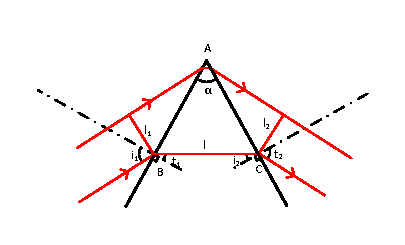
\includegraphics[width=0.6\textwidth]{feixe}
	\caption{Trajeto de um feixe luminoso paralelo num prisma. \label{fig:feixe}} 
\end{figure}

\begin{equation}
	\label{eq:sin_alpha}
	\frac{\sin \alpha}{l}= \frac{\sin (\pi/2 - t_1)} {AC}=\frac{\cos t_1} {AC}
\end{equation}

e atendendo a que $l_2= AC \cos t_2$, a Eq. (\ref{eq:37}) pode ser simplificada para 

\begin{equation}
	\label{eq:delt_lamd}
	\frac{\ud \delta}{\ud \lambda}  =  \frac{\ud n}{\ud \lambda} \frac{l}{l_2}
\end{equation}

Assim, uma pequena variação de comprimento de onda $\Delta \lambda$ produz uma variação do ângulo de desvio $\Delta \delta$  tal que 

\begin{equation}
	\label{eq:Delt_delta}
	\Delta \delta =  \frac{\ud n}{\ud \lambda} \frac{l}{l_2} \Delta \lambda 
\end{equation}

O critério de Rayleigh para que dois comprimentos de onda estejam resolvidos, i.e. possam ser detectados separadamente, é que o máximo de intensidade (de ordem $n \ge 1$) de um deles coincida com o mínimo de intensidade do outro (Figura \ref{fig:gauss})

\begin{figure}[ht]  \centering 
	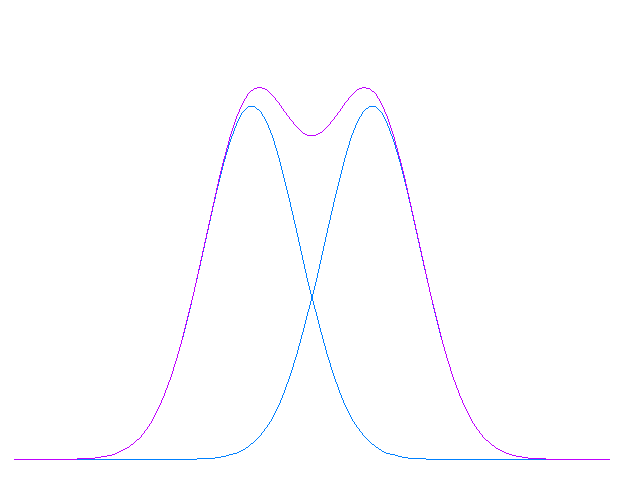
\includegraphics[width=0.6\textwidth]{gauss}
	\caption{Critério de Rayleigh da resolução de duas riscas espetrais (a vermelho a soma da intensidade das riscas. \label{fig:gauss}} 
\end{figure}

Pelas leis de difração, o primeiro mínimo de intensidade da figura de difração de uma fenda de largura $l_2$ dista angularmente do máximo principal de:  $\sin \theta = \lambda/l_2$.
Para dois comprimentos de onda muito próximos, $\sin  \theta \approx \theta $, que neste caso é o desvio angular $\Delta \delta$. Assim $\Delta \delta= \lambda / l_2$ e obtém-se para a resolução do prisma: 

~\begin{equation}
	\label{eq:resolup}
	R_\lambda  =  \frac{\lambda}{\Delta \lambda} = l \left(\frac{\ud n}{\ud \lambda} \right )_\lambda 
\end{equation}


\large{Bibliografia}\small\\
\emph{Óptica} (2.ª ed.), Eugene Hecht, Fund. Calouste Gulbenkian, 2002.


\end{document} 